\documentclass{article}
\usepackage[utf8]{inputenc}
\usepackage[spanish]{babel}
\usepackage{listings}
\usepackage{graphicx}
\graphicspath{ {images/} }
\usepackage{cite}

\begin{document}

\begin{titlepage}
    \begin{center}
        \vspace*{1cm}
            
        \Huge
        \textbf{Proyecto Final}
            
        \vspace{0.5cm}
        \LARGE
         Los Primeros Pasos
            
        \vspace{1.5cm}
            
        \textbf{Michael Stiven Zapata Giraldo}
            
        \vfill
            
        \vspace{0.8cm}
            
        \Large
        Despartamento de Ingeniería Electrónica y Telecomunicaciones\\
        Universidad de Antioquia\\
        Medellín\\
        Marzo de 2021
            
    \end{center}
\end{titlepage}

\tableofcontents
\newpage
\section{Introduccion}\label{intro}

Este es la primer parte de la planeacion del proyecto final para la materia de Informatica II, donde se introducirá de forma muy general como sera´el proyecto final, y es importante aclarar que como es el primer paso de este proyecto muy seguramente cambiaran muchas ideas y formas de plananear imagenes de objetivos en este proyecto.  

\section{Batalla Universal} \label{contenido}
Batalla Universal será un juego con tematica de galaxias, el cual pretenderá llegar a un nivel ganador, pero antes de...se deberá pasor por medio de tres niveles, los cuales se supone que cada vez cada nivel sera mas compliacdo que el nivel inmediatamente anterior, la idea es que a medida que vaya gastando municiones vayan apareciendo ayudas para recargar sus municiones, de igual manera a medida que al jugador vaya disminuyendo su nivel de vida apareceran recargar de sus vida para qyue este las alcance y pueda recuperar su vida y pues  te esta manera no pierda el juego. 

Debido a que este es proyecto final pues tendra seguramente de muchos tipos de datos de acuerdo a la necesidad de la interfaz grafica y del uso del juego como uso de las teclas, nivel de vida y municiones, cantidad de enemigos, nivel general ubicacion, tamaño de la pantalla y cosas asi...por lo que los datos numerico podrian ser int, float, double, en fin. Ademas, se otros datos para tipo texto que se usaran por ejemplo para el ingreso y registro de usuarios.

Como plantillas a proponer para este juego se podria proner las siguientes:

-Una para las balas, con atributos llamados radio, ybala, xbala, velybala, velxbala, aybala y como metodos moviminentoeny, y actulizarposicion.

-Una plantilla para desarrollo del campo del juego, donde las propuestas a los atributos serian inicialmente naves, inicialnaves, cont, conta2, vidas, niveldevida, nivel, contadorl6, bandera, banderaestatica, contador, jugador, naveplatillo, tercerenemigo, serialcomunicacion, bala, vidaAyuda. Y como metodo uno llamado actualizar.

-enemigo3, plantilla o clase que tendria los atributos de posx, posy, radio, acel,velx, con el metodo calposicion.

-enemigos seria una plantilla a proponer con los metodos  movimientosenemigosy actulizarmovimiento, y cuyos atributos serian posx, posy, velyenemigos,aceleracionyenemigos

Habra como prpuesta otras clases o plantillas como jugador, login, menu, municion, navedos, que se explicaran mas adelante debido a que en esta parte del proyecto seria un tanto inncesario entrar en este tipo de detalles, por lo que se informa de manera muy general lo que se pretende como proyecto final.


Ademas agregar que esta la posibilidad de que el jugador elija el tipo de nave con que quiere iniciar el juego para la "Batalla Universal".

Tambien como propuesta es que para el uso del arduino se maneje un semaforo para el uso o advertencia  de la cantidad de vidas disponible indicado que  en verde tiene suficientes cantidad de vida, amarillo para un tanto de la mitad y rojo pues que sus vidas se agotan. Tambein se puede disponer de otro arduino para un manejo de control para un segundo jugador, pues se sabe que uno de los requisitos es la parte de multijugador.


Para tener en cuenta se trabajara con la version de QT 5.12.2, en un portatil modelo con modelo LAPTO-76I56HDB, con procesador Intel CoreI5-6200U CPU @ 2.30GHz 2.4GHz y con SO de 64 bits y memoria RAM de 6.00 GB.
\subsection{Citación}


Curso de programacion en QT,Curso de programación con qt.\\\\

Guía aprender programar videojuegos con C++, http://razonartificial.com/2012/02/guia-aprender-programar-videojuegos-con-cpp/



En la sección \ref{imagenes}, se presentará como añadir ilustraciones al texto.

\section{Inclusión de imágenes} \label{imagenes}

En la Figura (\ref{fig:cpplogo}), se presenta una propuesta de tres para la eleccion de la nave como jugador.

\begin{figure}[h]
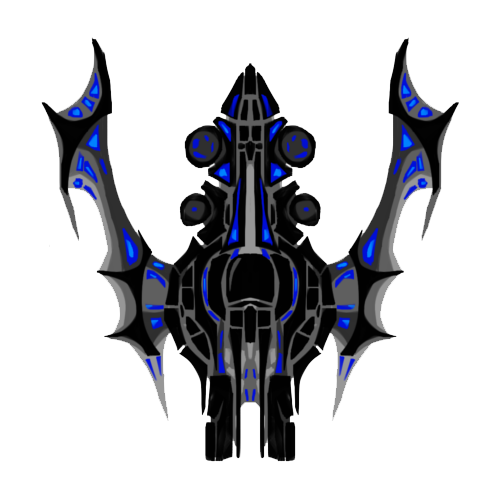
\includegraphics[width=4cm]{Nave.png}
\centering
\caption{Nave jugador de "Batalla Universal"}
\label{fig:cpplogo}
\end{figure}



\bibliographystyle{IEEEtran}
\bibliography{references}

\end{document}
